%% =============================================================================
%% Binary Decision Trees -- the CPS question that was on the final until it was
%% replaced by "Short Circuits" (draft_shortcircuit.tex) for being too hard.
%%
%% This is the copy AS IT WAS INLINED in exam_final.tex at the moment of
%% removal. It differs from q/bdt.tex, which is the earlier standalone fragment:
%%   - q/bdt.tex has "pictured by the BDT:" captions on the tikz diagrams and a
%%     "you need only fill in the three results" line that this copy lacks;
%%   - this copy has \vspace tweaks around the staged compress boxes for page
%%     fitting, and smaller solution boxes.
%% Neither is strictly newer -- keep both until you decide which to revive.
%% =============================================================================

\titledquestion{Binary Decision Trees}

\textbf{Binary Decision Trees}

We are interested in the problem of checking membership of a bit string in sets
of bit strings of length $n$. We are going to represent bit strings as values of
the type \code{bit list} in SML, where we have:

\begin{codeblock}
  datatype bit = One | Zero

  type bitstring = bit list
\end{codeblock}

So for instance, we might be interested if the bit string 0110 is in the set $\{
0000, 1100, 1101 \}$. This would be the same as implementing a function of type
\code{bitstring list -> bitstring -> bool}.

A naive way of doing this is to literally check list membership. For instance,
we might check every bit string in our set
\code{[[One, Zero], [Zero, Zero]]}, by comparing it to our bitstring-to-be-queried.

This can be enormously slow, however, because we might have to check potentially
$2^n$ many bit strings, for bit strings of length $n$! We can do much
better, by following the principle of a DFA, and making branching choices
by reading each character. This data structure is called a \textit{binary decision tree}.

Consider the following datatype:\footnote{Which is isomorphic to a \code{bool shrub}, for
those of you keeping track at home.}
\begin{codeblock}
  datatype bdt =
      Final of bool
    | Choice of bdt * bdt
\end{codeblock}

We think of each \code{Choice} node as having a \textbf{left child where the next character
is \code{0}}, and a \textbf{right child where the next character is \code{1}}. A
\code{Final} node represents whether the bit string leading to it is
in the set or not.

\textbf{Definition.} A value \code{b : bdt} is called \textbf{$n$-full} if
any path from the root to a \code{Final} node has length $n$. You can think of
it as representing a set of bit strings of length $n$.

For instance, this is a valid 2-full BDT:

\begin{center}
  \begin{tikzpicture}[
    level 1/.style={sibling distance=30mm},
    level 2/.style={sibling distance=15mm}
  ]
    \node {$\cdot$}
      child{node {$\cdot$}
        child{node {\code{false}}}
        child{node {\code{true}}}
      }
      child{node {$\cdot$}
        child{node {\code{false}}}
        child{node {\code{true}}}
      }
    ;
  \end{tikzpicture}
\end{center}

which represents the set of bit strings $\{ 01, 11 \}$.

\newpage

\begin{parts}
  \part[5]\hfill

    Write a function \code{check} with the following specification:
    \spec
      {check}
      {\code{bdt -> bitstring -> bool}}
      {\code{bdt} is $n$-full, and \code{List.length bs} $\eeq$ \code{n}}
      {\code{check bdt bs} $\eeq$ \code{b}, where \code{b} is the contents of
      the \code{Final} node reached by reading the bits of \code{bs}.
      }

    \begin{solutionorbox}[15em]
      \begin{codeblock}
        fun check bdt bs =
          case (bdt, bs) of
            (Final b, []) => b
          | (Choice (l, r), Zero::bs) => check l bs
          | (Choice (l, r), One::bs) => check r bs
      \end{codeblock}
    \end{solutionorbox}

  \part[5]\hfill

    We will also need to \textbf{partition} a list according to a predicate:
    true means left, false means right. For funsies, we will do it in CPS.

    \spec
      {partition}
      {\\ {\small\code{('a -> bool) -> 'a list -> ('a list * 'a list -> 'b) -> 'b}}}
      {\code{p} is total}
      {\code{partition p L k} $\eeq$ \code{k (A, B)}, where \code{A} holds the
      elements of \code{L} satisfying \code{p}, \code{B} holds the rest, and both
      preserve the order they had in \code{L}.}

    For instance, \code{partition (fn x => x mod 2 = 0) [1, 2, 3] (fn x => x)}
    evaluates to \code{([2], [1, 3])}.

    \begin{constraint}
      \code{partition} must be written in CPS.
    \end{constraint}

    \newpage

    \begin{solutionorbox}[16em]
      \begin{codeblock}
        fun partition p [] k = k ([], [])
          | partition p (x :: xs) k =
              partition p xs (fn (l, r) =>
                if p x then k (x :: l, r)
                else k (l, x :: r))
      \end{codeblock}

      The recursive call is made first, and its continuation receives the
      partition of the tail; we then place \code{x} into whichever side
      \code{p x} selects before handing the result to \code{k}.
    \end{solutionorbox}

  \part[3]\hfill

    Now, write a function \code{partition_bstrs} to partition a list of bit
    strings into ones which start with \code{One} and ones which start with
    \code{Zero}.

    \spec
      {partition_bstrs}
      {\code{bitstring list -> (bitstring list * bitstring list -> 'a) -> 'a}}
      {\code{bstrs} is a list of non-empty bit strings}
      {\code{partition_bstrs bstrs k} $\eeq$ \code{k (L, R)} such that
        \code{L} contains all bit strings in \code{bstrs} starting with a 0, and
        \code{R} contains all bit strings in \code{bstrs} starting with a 1.
      }

    \begin{constraint}
      You may not use the \code{fun} keyword, and you are allowed a single
      \code{fn} expression.
    \end{constraint}

    \begin{solutionorbox}[12em]
      \begin{codeblock}
        val partition_bstrs =
          partition
            (fn Zero :: _ => true
              | One  :: _ => false
            )
      \end{codeblock}

      \code{partition} applied to just its predicate is already the function we
      want --- the remaining two arguments (the list and the continuation) are
      supplied by the caller.
    \end{solutionorbox}

  \begin{EnvUplevel}
    However, checking can be a little redundant. Suppose that our set of
    bit strings is the set $\{ 00, 01, 10, 11 \}$. Then,
    we could do the work to query this set, or we could
    just observe that the answer is always \code{true}!

    This is because this set contains every single bit string of length
    2. In other words, as an $2$-full tree, our BDT looks like this:

    \begin{center}
      \begin{tikzpicture}[
        level 1/.style={sibling distance=27mm},
        level 2/.style={sibling distance=13mm}
      ]
        \node {$\cdot$}
          child{node {$\cdot$}
            child{node {\code{true}}}
            child{node {\code{true}}}
          }
          child{node {$\cdot$}
            child{node {\code{true}}}
            child{node {\code{true}}}
          }
        ;
      \end{tikzpicture}
    \end{center}

    but it may as well be described as the following tree:

    \vspace{10pt}

    \begin{center}
      \code{true}
    \end{center}

    \vspace{10pt}

    This is another way of saying that we can do some compression!

    \textbf{Definition.} A binary decision tree \code{bdt : bdt} is
    \textit{compressed} if the values \code{Choice (Final true, Final true)} and
    \code{Choice (Final false, Final false)} never appear in it anywhere.
  \end{EnvUplevel}



  \part[12]\hfill

    Now, let's get to the task of constructing our compressed BDT!

    Write a function \code{compress} with the specification:

    \spec
      {compress}
      {\code{int -> bitstring list -> bdt}}
      {\code{bstrs} is a list of unique bit strings, such that each bit string \code{bs} has
      that \code{List.length bs = n}}
      {\code{compress n bstrs} $\eeq$ the compressed BDT that
      represents the set of bit strings \code{bstrs}}

    \vspace{80pt}

    SPACE INTENTIONALLY LEFT BLANK -- KEEP READING

    \newpage

    I will use the shorthand of surrounding a bit string with curly braces to
    mean the corresponding SML value. For instance, \code{\{110\}} means
    \code{[One, One, Zero]}.

    Then, we should have the following compressed BDTs, visualized:
    \begin{itemize}
      \item \code{compress 1 []} $\eeq$ \code{Final false}

      \begin{center}
        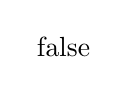
\begin{tikzpicture}[
          level distance=8mm,
          level 1/.style={sibling distance=50mm},
          level 2/.style={sibling distance=30mm},
          level 3/.style={sibling distance=15mm}
        ]
          \node {\code{false}}
          ;
        \end{tikzpicture}
      \end{center}
      \vspace{5pt}
      \item \code{compress 1 [\{0\}, \{1\}]} $\eeq$ \code{Final true}

      \begin{center}
        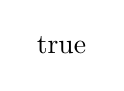
\begin{tikzpicture}[
          level distance=8mm,
          level 1/.style={sibling distance=50mm},
          level 2/.style={sibling distance=30mm},
          level 3/.style={sibling distance=15mm}
        ]
          \node {\code{true}}
          ;
        \end{tikzpicture}
      \end{center}
      \vspace{5pt}
      \item \code{compress 1 [\{0\}]} $\eeq$ \code{Choice (Final true, Final false)}

      \begin{center}
        \begin{tikzpicture}[
          level distance=8mm,
          level 1/.style={sibling distance=50mm},
          level 2/.style={sibling distance=30mm},
          level 3/.style={sibling distance=15mm}
        ]
          \node {$\cdot$}
            child{node{\code{true}}}
            child{node{\code{false}}}
          ;
        \end{tikzpicture}
      \end{center}
      \vspace{5pt}
      \item \code{compress 1 [\{1\}]} $\eeq$ \code{Choice (Final false, Final true)}

      \begin{center}
        \begin{tikzpicture}[
          level distance=8mm,
          level 1/.style={sibling distance=50mm},
          level 2/.style={sibling distance=30mm},
          level 3/.style={sibling distance=15mm}
        ]
          \node {$\cdot$}
            child{node{\code{false}}}
            child{node{\code{true}}}
          ;
        \end{tikzpicture}
      \end{center}
      \vspace{5pt}
      \item \code{compress 2 [\{00\}, \{01\}, \{10\}, \{11\}]} $\eeq$ \code{Final true}

      \begin{center}
        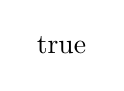
\begin{tikzpicture}[
          level distance=8mm,
          level 1/.style={sibling distance=50mm},
          level 2/.style={sibling distance=30mm},
          level 3/.style={sibling distance=15mm}
        ]
          \node {\code{true}}
          ;
        \end{tikzpicture}
      \end{center}
      \vspace{5pt}
      \item \code{compress 3 [\{000\}, \{110\}, \{101\}, \{100\}]} $\eeq$
      \begin{codeblock}
        Choice
          ( Choice
              (Choice (Final true, Final false), Final false),
            Choice
              (Final true, Choice (Final true, Final false))
          )
      \end{codeblock}
    \end{itemize}
    which denotes the BDT of
    \begin{center}
      \begin{tikzpicture}[
        level distance=8mm,
        level 1/.style={sibling distance=50mm},
        level 2/.style={sibling distance=30mm},
        level 3/.style={sibling distance=15mm}
      ]
        \node {$\cdot$}
          child{node {$\cdot$}
            child{node {$\cdot$}
              child{node {\code{true}}}
              child{node {\code{false}}}
            }
            child{node {\code{false}}}
          }
          child{node {$\cdot$}
            child{node {\code{true}}}
            child{node {$\cdot$}
              child{node {\code{true}}}
              child{node {\code{false}}}
            }
          }
        ;
      \end{tikzpicture}
    \end{center}

    \newpage

    Reproduced for your convenience: write a function \code{compress} with the
    spec:

    \spec
      {compress}
      {\code{int -> bitstring list -> bdt}}
      {\code{bstrs} is a list of unique bit strings, such that each bit string \code{bs} has
      that \code{List.length bs = n}}
      {\code{compress n bstrs} $\eeq$ the compressed BDT that
      represents the set of bit strings \code{bstrs}}

    You may assume that you are given \code{pow : int * int -> int}, such that
    \code{pow (n, k)} $\eeq$ $n^k$, and \code{tl : 'a list -> 'a list}, which
    obtains the rest of a list after the first element (if possible), and raises an exception otherwise.

    \textbf{Hint:} There are $2^n$ bit strings of length \code{n}. You should use
    \code{partition_bstrs} and \code{tl}.

    \begin{codeblock}
      fun compress (n : int) (bstrs : bitstring list) =
        if List.length bstrs = pow (2, n) then
    \end{codeblock}
    \vspace{-0.2cm}
    \begin{solutionorbox}[4em]
      \begin{codeblock}
        Final true
      \end{codeblock}
    \end{solutionorbox}

    \begin{codeblock}[autogobble=false]
  else if List.length bstrs = 0 then
    \end{codeblock}
  \vspace{-0.6cm}

    \begin{solutionorbox}[4em]
      \begin{codeblock}
        Final false
      \end{codeblock}
    \end{solutionorbox}

    \begin{codeblock}[autogobble=false]
  else
    \end{codeblock}
    \vspace{-0.6cm}
    \begin{solutionorbox}[20em]
      \begin{codeblock}
            partition_bstrs bstrs (fn (l, r) =>
              Choice
                ( compress (n - 1) (List.map tl l)
                , compress (n - 1) (List.map tl r)
                )
            )
      \end{codeblock}
    \end{solutionorbox}

  % \part[5]\hfill

  %   Write and solve a recurrence which denotes the \textbf{work} of \code{compress},
  %   in terms of the input value \code{n}, assuming that preconditions hold.

  %   % state the work of pow and partition_strs

  %   Show your work.

  %   \begin{solutionorbox}[19em]
  %     $W_{\code{compress}}(0) = c_0$
  %     $W_{\code{compress}}(n) = O(2^n) + 2 \cdot W_{\code{compress}}(n - 1)$

  %     \begin{align*}
  %       W_{\code{compress}}(n) \\
  %       &= O(2^n) + 2 \cdot W_{\code{compress}}(n - 1) \\
  %       &= O(2^n) + 2 \cdot (O(2^{n - 1}) + W_{\code{compress}}(n - 2)) \\
  %       &= O(2^n) + O(2^n) + W_{\code{compress}}(n - 2)
  %     \end{align*}

  %     This evaluates to $\Sum_{i = 0}^n O(2^n) = O(n2^n)$.
  %   \end{solutionorbox}

  % \part[5]\hfill

  %   Write and solve a recurrence which denotes the \textbf{span} of \code{compress},
  %   in terms of the input value \code{n}, assuming that preconditions hold.

  %   Assume that \code{partition_strs} partitions approximately evenly, and runs in
  %   linear time in its input list length.

  %   Show your work.

  %   \begin{solutionorbox}[19em]
  %     $S_{\code{compress}}(0) = c_0$
  %     $S_{\code{compress}}(n) = O(2^n) + S_{\code{compress}}(n - 1)$

  %     \begin{align*}
  %       S_{\code{compress}}(n) \\
  %       &= O(2^n) + \cdot S_{\code{compress}}(n - 1) \\
  %       &= O(2^n) + O(2^{n - 1}) + S_{\code{compress}}(n - 2)
  %     \end{align*}

  %     This evaluates to $1 + 2 + ... + 2^n = O(2^n)$.
  %   \end{solutionorbox}

  % \newpage

  % \part[10]\hfill

  %   Write a function \code{insert} which satisfies the following
  %   specification:
  %   \spec
  %     {insert}
  %     {\code{bdt -> char list -> bdt}}
  %     {\code{bt} is a compressed BDT and \code{cs} is a bit string that cannot
  %     be shorter than any bit string in \code{bt}}
  %     {\code{insert bt cs} evaluates to the BDT which now contains
  %     the bit string \code{cs}, but is otherwise equivalently compressed}

  %   \begin{solutionorbox}[30em]
  %     \begin{codeblock}
  %       fun insert (bt : bdt) (cs : char list) =
  %         case (bt, cs) of
  %           (_, []) => Final true
  %         | (Choice (L, R), #"0"::cs') =>
  %             Choice (insert L cs', R)
  %         | (Choice (L, R), #"1"::cs') =>
  %             Choice (L, insert R cs')
  %         | (Final b, #"0"::cs') =>
  %             Choice (insert L cs', Final b)
  %         | (Final b, #"1"::cs') =>
  %             Choice (Final b, insert R cs')
  %         | _ => raise Precondition
  %     \end{codeblock}
  %   \end{solutionorbox}

  \part[5]\hfill

    Now, we can compress our bit string sets, and query them.

    Consider the following such function:

    \begin{codeblock}
      fun query (n : int) (bstrs : bitstring list) (bs : bitstring) =
        check (compress n bstrs) bs
    \end{codeblock}

    Suppose we are interested in repeat queries to the same set of bit strings.
    There is an inefficiency in this code. Rewrite \code{query} to perform better
    in that case.

    \begin{solutionorbox}[15em]
      \begin{codeblock}
        fun query (n : int) (bstrs : bitstring list) =
          let
            val bdt = compress n bstrs
          in
            fn bs => check bdt bs
          end
      \end{codeblock}
    \end{solutionorbox}
\end{parts}

\newpage

